\documentclass[a4]{article}

\usepackage{graphicx}
\usepackage{amsmath, amsfonts, geometry, float, listings, enumerate, multicol}
\usepackage{multicol, float, color, colortbl}
\usepackage{tikz, titlesec, parskip, pgfplots, filecontents}
\usepackage{hyperref}
\usepackage{amsmath}
\usepackage{tikz, titlesec, parskip}
\usepackage{tikz,pgfplots}
\usepackage[americanvoltages,fulldiodes,siunitx]{circuitikz}
\usetikzlibrary{shapes,arrows}
\usepackage{enumitem}
\titleformat*{\subsubsection}{\LARGE\bfseries}
\usepackage{subcaption}
\usepackage{caption}
\titlespacing{\section}{0pt}{10pt}{0pt}
\titlespacing{\subsection}{0pt}{10pt}{0pt}
\titlespacing{\subsubsection}{0pt}{10pt}{0pt}


\usetikzlibrary{calc,patterns,through}
\newcommand{\arcangle}{%
	\mathord{<\mspace{-9mu}\mathrel{)}\mspace{2mu}}%
}

\renewcommand{\baselinestretch}{1.4}
 \geometry{
 a4paper,
 total={170mm,257mm},
 left=20mm,
 top=20mm,
 }
\usepackage{fancyhdr}
\usepackage{indentfirst}
\pagestyle{fancy}
\fancyhf{}
\rhead{\textbf{پردازش تصاویر دیجیتال}}
\lhead{\textbf{تمرین سری پنجم}}
\cfoot{(\space \space \space \space \textbf{\thepage}  \space \space \space)}
\renewcommand{\headrulewidth}{1pt}
\renewcommand{\footrulewidth}{1pt}

 
\usepackage{xepersian}
\setlatintextfont{Times New Roman}
\settextfont{XB Niloofar}
\setdigitfont{XB Niloofar}
\DefaultMathsDigits

\makeatletter
\bidi@patchcmd{\@Abjad}{آ}{الف}
{\typeout{Succeeded in changing آ into الف}}
{\typeout{Failed in changing آ into الف}}
\makeatother
\PersianAlphs

\begin{document}
\begin{minipage}{0.6\textwidth}
\begin{bf}
	\begin{center}
		به نام خدا\\
		\vspace{0.25cm}
		دانشگاه صنعتی شریف\\
		\vspace{0.25cm}
		دانشکده مهندسی برق\\
		\vspace{0.5cm}
	
	\large
	دکتر عمادالدین فاطمی‌زاده - پردازش تصاویر دیجیتال \\
	نیم سال دوم
	۱۴۰۱-۱۴۰۰\\
	\Large
	\vspace{0.4cm}
	تمرین عملی سری پنحم\\
	\end{center}
\end{bf}
\normalsize
\end{minipage} \hfill
\begin{minipage}{0.35\textwidth}
\begin{flushleft}
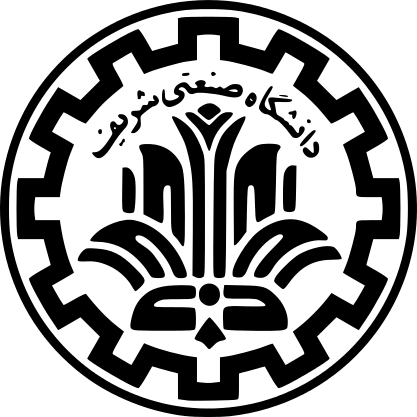
\includegraphics[width=0.5\textwidth]{Shariflogo.png}\\ \large
\end{flushleft}

 \end{minipage}
\\

\rule[0.1\baselineskip]{\textwidth}{1pt}

\large
\section*{
لطفاً به نکات زیر توجه بفرمایید: (رعایت نکردن این موارد باعث کاهش نمره می‌شود.)
}

\begin{enumerate}
	\item 
نتایج و پاسخ های خود را در یک فایل با فرمت zip به نام
\LR{HW$5$-Name-StudentNumber}
 در سایت  
\href{https://quera.org/course/add_to_course/course/10598/}{\lr{Quera}} 
 قرار دهید. همچنین فایل پایتون یا متلب خود را به همان نام در قسمت مخصوص به خود آپلود کنید.
\item 
کسب نمره کامل در هر سوال مستلزم تحویل  
\textbf{کدها (40 نمره)}
 و
\textbf{توضیحات (30 نمره)}
و
\textbf{نتایج (30 نمره)}
 می‌باشد. 
\item 
کدهای شما تماماً باید توسط خودتان نوشته شده باشند. هرگونه استفاده از کد دیگران، اعم از دوستان و اینترنت، به هر شکل ممکن، تقلب محسوب می‌شود و نمره تمام تمرینات جاری و تمام تمرینات قبلی صفر خواهد شد. با اجرای این کدها باید همان نتایجی که فرستاده اید قابل بازیابی باشند. برنامه شما باید به گونه‌ای باشد که بدون نیاز به هیچ تغییری قابل اجرا باشد، در غیر این‌ صوررت هیچ نمره‌ای تعلق نخواهد گرفت. 
\item 
برای تمام سؤالات، باید جزئیات روشی که استفاده کرده‌اید را توضیح دهید و نتایجی که گرفته‌اید را ارائه دهید. این توضیحات می‌تواند در یک فایل  pdf  و یا در یک فایل  ipynb باشد. در توضیحات، باید اشاره کامل به کارهایی که انجام داده‌اید بنمایید به طوری که یک شخص آگاه از موارد درس بتواند به آسانی متوجه کاری که شما انجام داده‌اید شود.
\item 
در طول ترم امکان ارسال با تاخیر پاسخ  همه‌ی تمارین تا سقف شش روز و در مجموع بیست و یک روز وجود دارد. پس از گذشت این مدت، پاسخ‌های ارسال‌شده پذیرفته نخواهند بود. همچنین، به ازای هر روز تأخیر غیر مجاز  بیست درصد از نمره تمرین به صورت ساعتی کسر خواهد شد.
\item 
 اگر از
\lr{Jupyter notebook} 
 استفاده می‌کنید، میتوانید خروجی‌ها‌ را پاک کنید تا حجم فایل تحویلی زیاد نشود.
\item 
مهلت تحویل: 
\item 
نام طراح هر سوال در زیر آن نوشته شده است و شما میتوانید سوالات خود را از طریق ایمیل یا تلگرام از طراح سوال بپرسید.
\\
ارسلان فیروزی:
\lr{Arsalan.firoozi@gmail.com } - \lr{@Arsalanfiroozi}
\\
سید سعید رضوی:
\lr{Saeedrazavi890@gmail.com} - \lr{@RazooIs}
\\
امیرحسین جوادی:
\lr{Javadiamirhosein.2000@gmail.com} - \lr{@Amirhosein\_javadi}

\end{enumerate}
\rule[0.1\baselineskip]{\textwidth}{1pt}

\clearpage
\section{\lr{Image Compression}}
\textbf{طراح :‌ سید سعید رضوی}
\vspace{0.5cm}
\\
در این سوال قصد کاهش حجم عکس
\lr{(compression)}
و بخش بندی 
\lr{(clustering)}
آن را به طور همزمان داریم.
ابتدا تصویر
\lr{q1.jpg}
 را بخوانید  و هیستوگرام مربوط به هر کانال را رسم  و به ترتیب با نام‌های 
\lr{hist\_r.jpg}،
\lr{hist\_g.jpg}
و
\lr{hist\_b.jpg}
 ذخیره نمایید. سپس با توجه به داده‌های هر هیستوگرام ، مقادیر بین $ 0 $ تا $ 255  $ را با یک مقدار مشخص کوانتیزیشن (این مقدار در حقیقت همان طول تقسیم بندی می‌باشد)، تقسیم بندی 
\lr{(quantize)}
 کنید. برای مثال اگر مقدار کوانتیزیشن برابر $ 32 $ باشد ، $ 8 $ بازه داریم و تمام مقادیری که در یک بازه مشخص هستند دقیقا به وسط آن بازه ارجاع داده  می‌شوند. این کار را برای تمام پیکسل‌ها و بر روی تمامی کانال‌ها انجام دهید و تصویر بخش بندی شده را با نام
\lr{clustered.jpg}
ذخیره نمایید.  هیستوگرام تصویر جدید را برای کانال های مختلف را با نام‌های
\lr{hist\_r\_clus.jpg}،
\lr{hist\_g\_clus.jpg}
و
\lr{hist\_b\_clus.jpg} 
ذخیره کنید. همچنین حجم اشغال شده تصویر جدید را با تصویر
\lr{q1.jpg}
مقایسه کنید و علتش را به صورت دقیق در گزارش ذکر کنید.
\\
(دقت شود اگر مقدار کوانتیزیشن رو از حدی بیشتر بگیرید تصویر نهایی با تصویر اصلی بسیار متفاوت می‌شود و اگر این مقدار را از حدی کمتر بگیرید نتیجه شما همچنان پر حجم  و پیاده سازی آن زمان‌بر می‌شود. مقدار بهینه این پارامتر را در گزارش خود ذکر کنید.)  
\\
نمونه از این بخش‌بندی در شکل زیر قابل مشاهده است: 
\begin{figure}[H]
	\centering
	\begin{subfigure}{.3\textwidth}
		\centering
		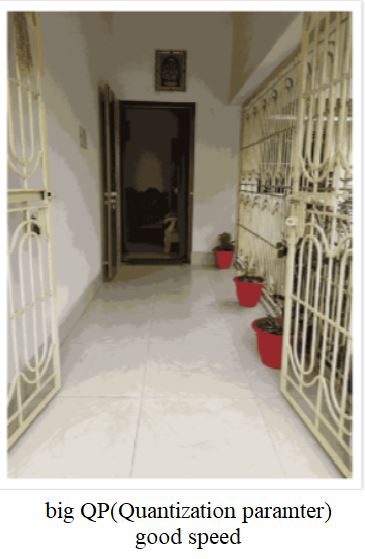
\includegraphics[width=.9\linewidth]{q1_3}
	\end{subfigure}%
	\begin{subfigure}{.3\textwidth}
		\centering
		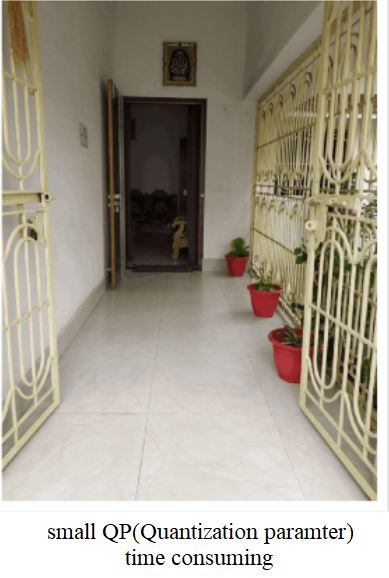
\includegraphics[width=.9\linewidth]{q1_2}
	\end{subfigure}
	\begin{subfigure}{.3\textwidth}
		\centering
		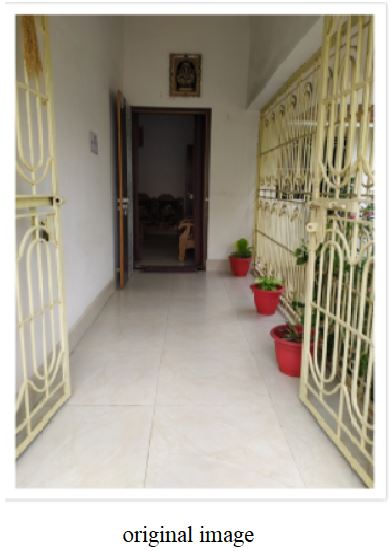
\includegraphics[width=.9\linewidth]{q1_1}
	\end{subfigure}
	\caption{}
\end{figure}
\section{\lr{Dynamic Programming}}
\textbf{طراح :‌ سید سعید رضوی}
\vspace{0.5cm}
\\
یکی از کاربرد‌های
\lr{laplacian pyramid}
(هرم لاپلاسین) در ساخت یک عکس بزرگتر با استفاده از چند عکس می‌باشد. در واقع اگر چند عکس که دارای نواحی مشترک می‌باشند داشته باشیم، میتوانیم با استفاده از هرم لاپلاسین در ناحیه مشترک، این عکس‌ها را به هم بچسبانیم. حال دو عکس زیر را در نظر بگیرید:
\begin{figure}[H]
	\centering
	\begin{subfigure}{.5\textwidth}
		\centering
		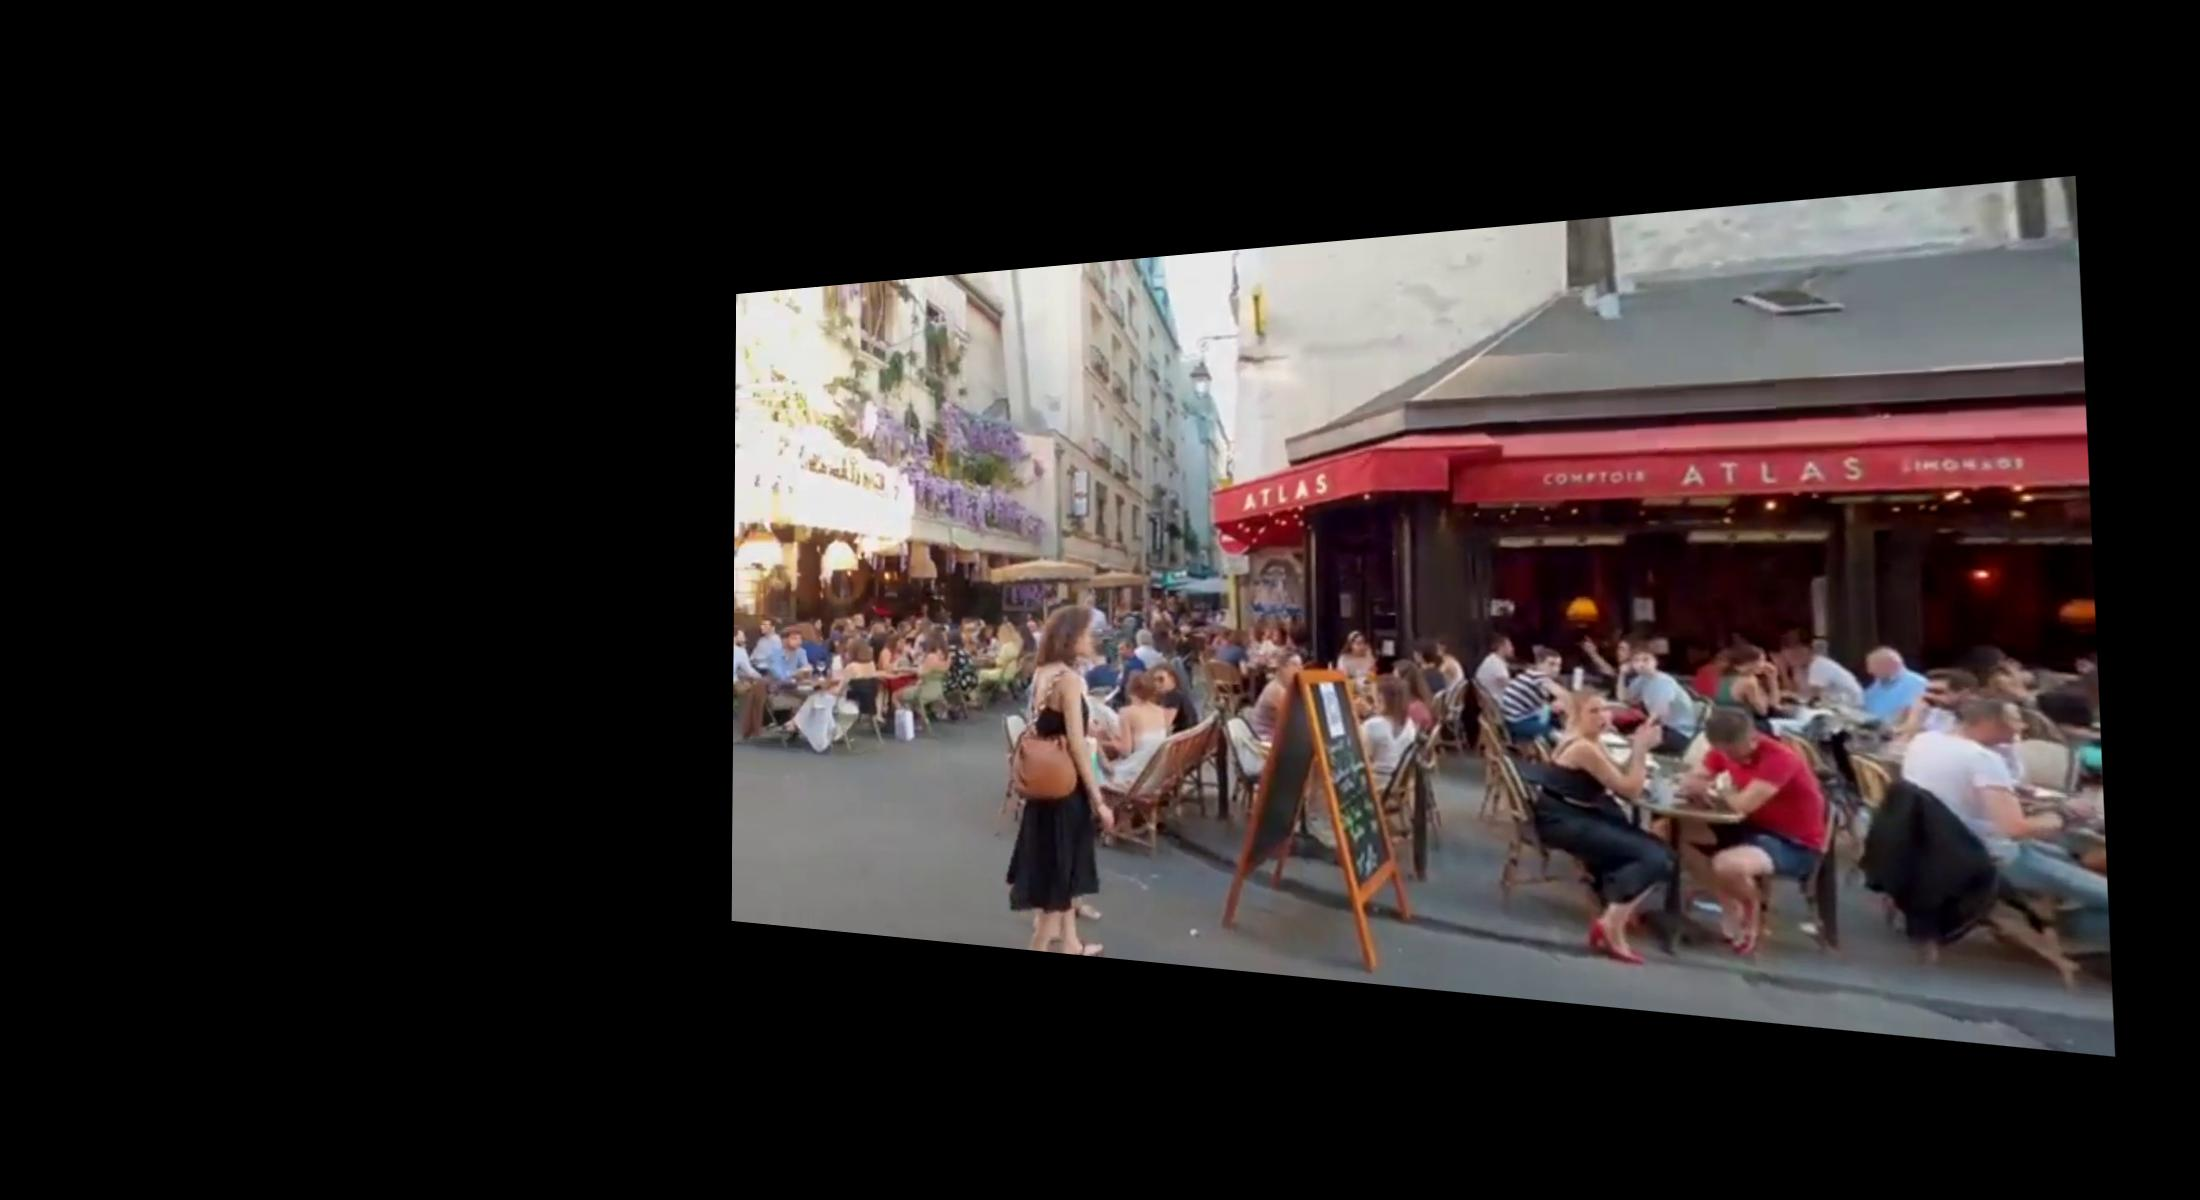
\includegraphics[width=.9\linewidth]{q2_1}
	\end{subfigure}%
	\begin{subfigure}{.5\textwidth}
		\centering
		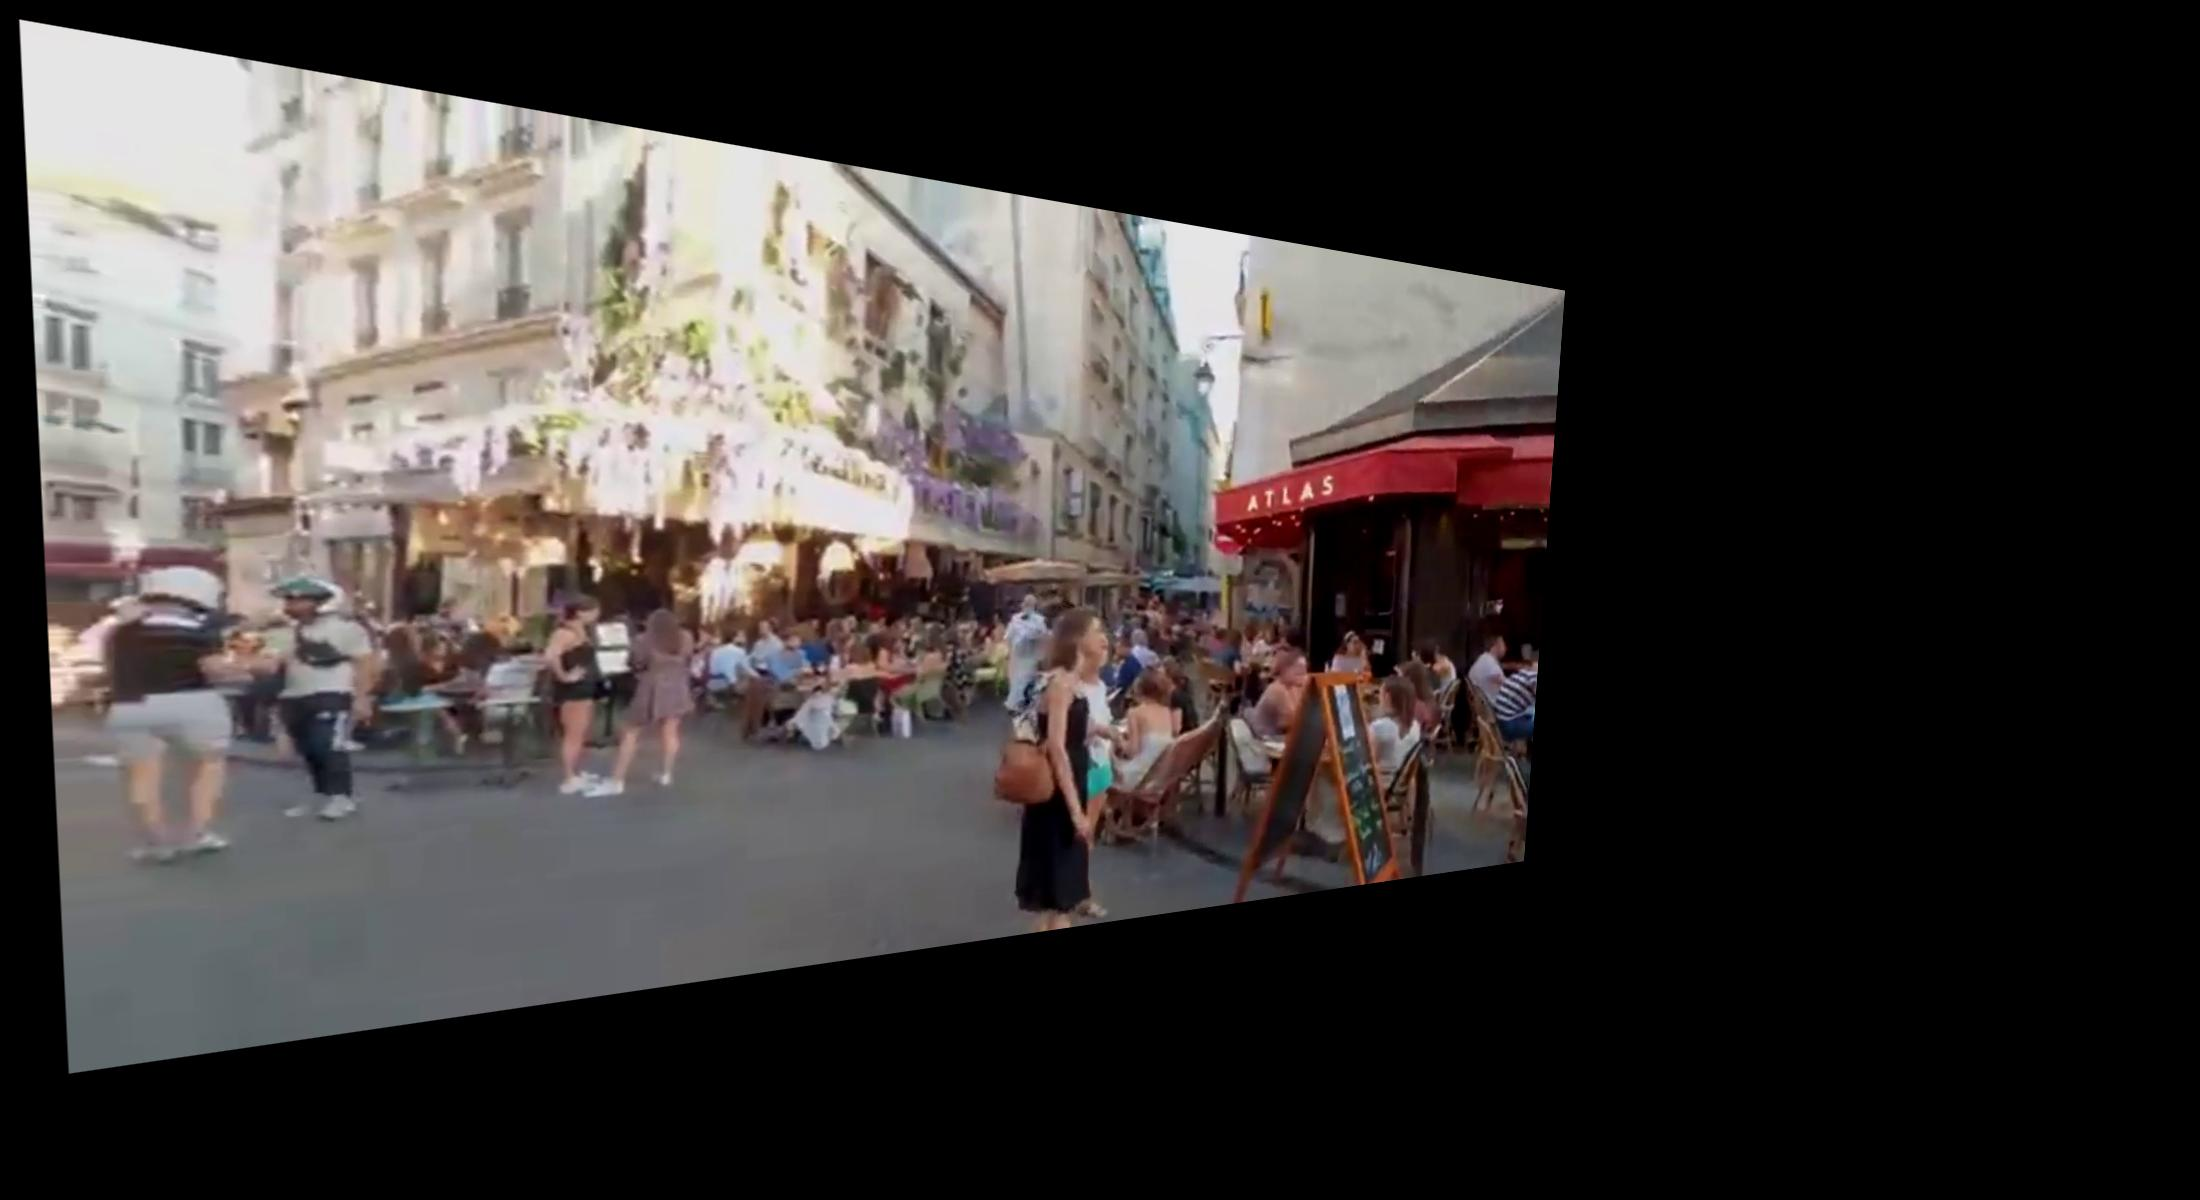
\includegraphics[width=.9\linewidth]{q2_0}
	\end{subfigure}
	\caption{}
\end{figure}
اگر بدون کمک از هرم لاپلاسین بخواهیم این دو تصویر را روی هم بیندازیم داریم: 
	\begin{figure}[H]
		\centering
		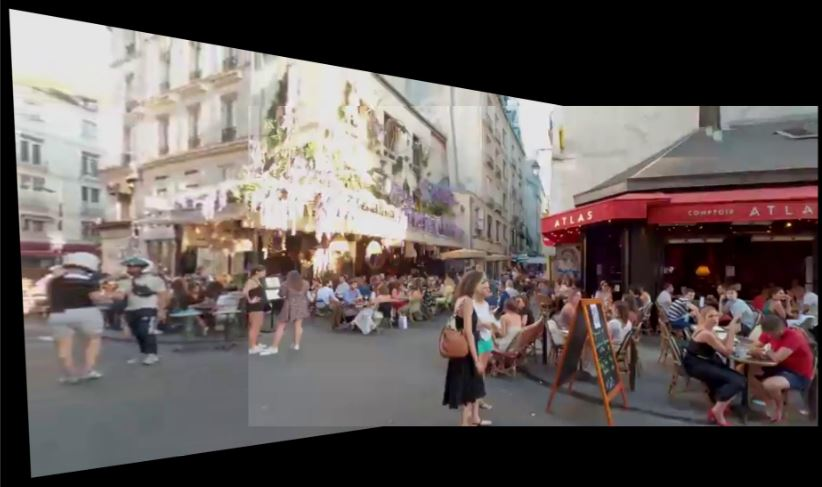
\includegraphics[width=0.6 \linewidth]{q2_2}
		\caption{
		}
		
	\end{figure}
همانطور که مشاهده می‌کنید تصویر حاصل کیفیت جالبی ندارد. به همین دلیل با استفاده از هرم لاپلاسین می‌توانید ترکیب دو تصویر را کمی طبیعی‌تر کنید. احتمالا اگر این کار را انجام دهید کیفیت تصویر نهایی نسبت به تصویر بالا بهتر شده اما باز هم مشخص است که تصویر نهایی شما ترکیب دو تصویر دیگر است‌. یکی از بهترین روش‌ها برای طبیعی‌تر کردن تصویر، پیدا کردن بهترین مرز جدایی این دو تصویر است‌. اسم این روش
\lr{minimum error boundary cut}
می‌باشد که با استفاده از برنامه نویسی پویا
\lr{(dynamic programming)}
بهترین مرز بین دو تصویر با ناحیه مشترک را پیدا میکند (برای مطالعه بیشتر درمورد این روش  می توانید 
این لینک 
\href{https://courses.engr.illinois.edu/cs445/fa2019/lectures/Lecture%2007%20-%20Texture%20Synthesis%20-%20CP%20Fall%202019.pdf}{این لینک}
و اسلاید‌های $ 29 $ تا $ 36 $ آن را مطالعه نمایید). 
در نهایت سعی کنید با پیدا کردن بهترین مرز جدایی و در آخر استفاده از هرم لاپلاسین تصویری بزرگتر از دو تصویر اولیه بسازید‌. همچنین در صورت پیدا کردن مرز بهینه در ناحیه اشتراک آن را در تصویری با نام
\lr{boarder.jpg}
 ذخیره نمایید. استفاده از هر روش دیگری که باعث رسیدن به نتیجه بهتر شود بلامانع است. نمره این سوال تا حد خوبی به نتیجه نهایی شما بستگی دارد. 
 تصویر نهایی را با نام 
\lr{res\_q2.jpg}
  ذخیره نمایید. 
\section{\lr{Wavelet}}
\textbf{طراح :‌ ارسلان فیروزی}
\vspace{0.5cm}
\\
در این سوال قصد داریم نویز موجود در تصویر
\lr{Q3.jpg}
 را به وسیله تبدیل
\lr{Wavelet} 
کاهش دهیم.
\begin{enumerate}
	\item 
از تصویر داده شده در $ 2 $ سطح تبدیل
	\lr{Wavelet}
 بر مبنای فیلتر
	\lr{Haar}
بگیرید و مطابق شکل زیر ضرایب بدست آمده را نمایش دهید:
	\begin{figure}[H]
		\centering
		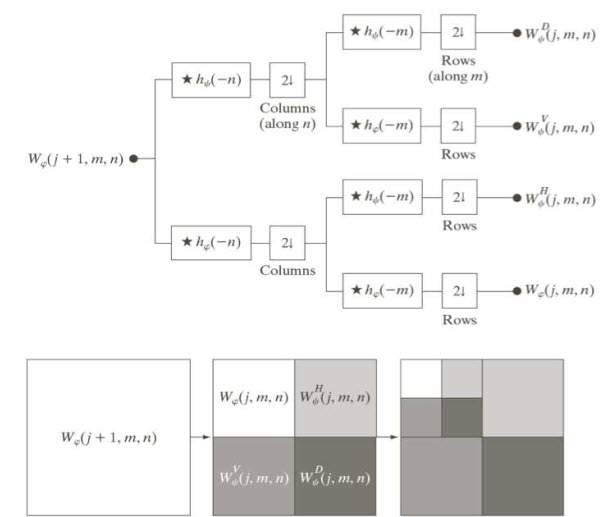
\includegraphics[width=0.7 \linewidth]{q3}
		\caption{
			\lr{One level of the wavelet decomposition}
		}
		\label{q3}
	\end{figure}
	\item 
با استفاده از روش
 \lr{VisoShrink}
 به یک مقدار آستانه مناسب برسید و ضرایب را از طریق هر دو روش 
 \lr{Soft} 
 و 
 \lr{Hard} 
 اصلاح کنید. سپس تصاویر را بازگردانی کنید و از مناسب بودن آستانه مطمئن شوید. 
	\item 
با استفاده از روش
 \lr{BayesShrink}
 به یک مقدار آستانه مناسب برسید و ضرایب را از طریق هر دو روش 
 \lr{Soft} 
و 
\lr{Hard} 
 اصلاح کنید. سپس تصاویر را بازگردانی کنید و از مناسب بودن آستانه مطمئن شوید. 
	\item 
با توجه به هیستوگرام ضرایب، در صورتی که سطح آستانه بزرگ در نظر گرفته شود چه تاثیری بر نتایج می‌‌گذارد؟ در صورتیکه سطح آستانه کوچک در نظر گرفته شود، چطور؟ نتایج با تحلیل خود را در گزارش بیاورید.
	
\end{enumerate}

\section{\lr{Shannon Source Coding Theorem}}
\textbf{طراح :‌ امیرحسین جوادی}
\vspace{0.5cm}
\\
در این قسمت می‌خواهیم با کدینگ منبع
\lr{(Source Coding)}
 آشنا شویم. برای مدل کردن منبع اطلاعاعات، باید به هر سمبل از منبع یک احتمال نسبت بدهیم. در نتیجه می توانیم منبع اطلاعاعات را به این صورت نمایش دهیم.
 \[X = \begin{pmatrix}
 	x_1 & x_2 & \dots & x_M\\
 	p_1 & p_2 & \dots & p_M
 \end{pmatrix}\]
 به عنوان مثال، اگر شما تصاویر سیاه و سفید تولید می‌کنید هر سمپل خروجی این منبع ، عددی بین $ 0 $ تا $ 255 $ است (در نتیجه 
 \lr{M = 256}
 ).
 مسأله‌ی کدینگ منبع آنست که می‌خواهیم یک نگاشت مانند
 \lr{$C$}
 از الفبای خروجی منبع به الفبای دوتایی
 \lr{$\mathcal{D} = \{0,1\}$}
 پیدا کنیم به گونه‌ای که طول متوسّط هر کلمه‌کد کمینه شود. به تعبیر دیگر اگر طول کلمه‌کد متناظر با سمبل
 \lr{$x\in\mathcal{X}$}
 را با
 \lr{$l(x)$}
 نشان دهیم، هدف آن است که
 \lr{$\mathbb{E}[l(X)]$}
 کمینه شود. 
 \\
 منبع اطلاعات زیر را در نظر بگیرید:
\lr{\[X = \begin{pmatrix}
		I_{x}=0 & I_{x}=50 & I_{x}=100 & I_{x}=150 & I_{x}=200 & I_{x}=250 & \text{otherwise}\\
		\frac{1}{2} & \frac{1}{32} & \frac{1}{8} & \frac{1}{16}& \frac{1}{32}& \frac{1}{4} & 0
	\end{pmatrix}\]}
\begin{enumerate}
	\item 
 کلمه کدها را برای منبع  $ X $ بسازید. کدینگ شما باید قابل بازیابی باشد و همچنین بهینه باشد. 
 	\item 
 	تابعی به نام 
 	\lr{InformationSource}
 	بسازید که تصویری (آرایه دو بعدی) به اندازه‌ی
 	 $ 28 \times 28 $
 	 به صورت 
 	 \lr{iid}
 	 تولید کند که توزیع احتمالی مانند توزیع احتمال منبع
 	 \lr{$X$}
 	 باشد.
 	 \item
 	 تابعی با عنوان
 	 \lr{SourceEncoder}
 	 بنویسید که در ورودی تصویر ساخته شده در قسمت قبل را در وروردی دریافت کند و در خروجی رشته از صفر و یک‌ها بدهد که کدشده‌ی تصویر ورودی است.
 	 \item 
 	 تابعی با عنوان
 	 \lr{SourceDecoder}
 	 بنویسید که در ورودی، دنباله‌ای از صفر و یک‌ها دریافت کند و در خروجی، تصویر متناظر را بدهد.   
 	 \item 
 	 درستی توابع
 	 \lr{SourceEncoder}
 	 و 
 	 \lr{SourceDecoder}
 	 را بررسی کنید. $ 10 $ تصویر تصادفی تولید کنید و مراحل کدگذاری و کدگشایی را روی این تصاویر اعمال کنید. آیا تصاویر ورودی و خروجی برابر شد؟ 
 	 \item 
 	 $ n = 1000 $ 
 	 تصویر تصادفی تولید کنید. برای هر تصویر طول رشته کدگذاری شده را بیابید. بردار‌ی به طول $ n $ به نام 
 	 \lr{L\_avg}
بسازید و خانه‌ی‌ $ i $ ام آن را میانیگن طول رشته کد $ i $ عکس اول قرار دهید. نمدار تغییرات این بردار را رسم کنید. انتظار دارید میانگین خواسته شده به چه عددی میل کند؟ 
\end{enumerate}
\section{\lr{Golomb Coding}}

\textbf{طراح :‌ ارسلان فیروزی}
\\
در این سوال از شما انتظار می‌رود که روش کدینگ 
	\lr{Golomb}
 را برای یک تصویر
  \lr{Grayscale} 
 دلخواه پیاده سازی کنید. از طریق تابع انکودینگ ابتدا تمام مقادیر پیکسل ها را با اعداد رندوم m انکود کنید. سپس از طریق تابع دیکود و همان مقادیر رندوم
  $ m $،
   مقادیر کد شده را دیکود کنید. با توجه به 
   \lr{Lossless }
   بودن فشرده سازی، انتظار داریم تصویر بدست آمده مطابق تصویر اولیه باشد.\\
از طریق کامنت خطوط کد را توضیح دهید.
\section{تئوری}
	مسائل روبرو از فصل هشتمِ کتاب درسی (ویرایش سوم) را حل کنید:
	 $ 1 $، $ 8 $، $ 10 $ و $ 18 $

\end{document}